\chapterimage{images/recycler/recycling.jpg}
\chapter{Recyclerview}
In 2014, Google released RecyclerView , via the Android Support package.
Developers can add the recyclerview-v7 to their projects and use RecyclerView. In this chapter, we will review RecyclerView from the ground up, starting with basic
operation.

Before you are able to use the recylceview,  open build.gradle (app) and add the dependencies needed.

\begin{xml}
    compile 'com.android.support:recyclerview-v7:+'
	compile 'com.android.support:cardview-v7:+'
\end{xml}

\section{What is a recyclerview}
The RecyclerView is a new ViewGroup that is prepared to render any adapter-based view. It is supposed to be the successor of ListView and GridView, and it can be found in the latest support-v7 version. One of the reasons is that RecyclerView has a more extensible framework, especially since it provides the ability to implement both horizontal and vertical layouts. Use the RecyclerView widget when you have data collections whose elements change at runtime based on user action or network events.

To use a recyclerview, you will need the following things:
\begin{enumerate}
	\item RecyclerView.Adapter - To handle the data collection and bind it to the view
	\item A layout file defining the row layout in the recyclerview. Just a note here: when you create the item layout of the RecyclerView don’t forget to add the following lines in the ViewGroup container of the layout. This lines of code will add the ripple effect to the RecyclerView elements.
	\begin{enumerate}
		\item  android:clickable="true"
		\item android:focusable="true"
		\item android:foreground="?android:attr/selectableItemBackground"
	\end{enumerate}
	\item LayoutManager - Helps positioning the items
	\item ItemAnimator - Helps with animating the items for common operations such as Addition or Removal of item
\end{enumerate}


\section{Components and Workflow}

\begin{figure}
	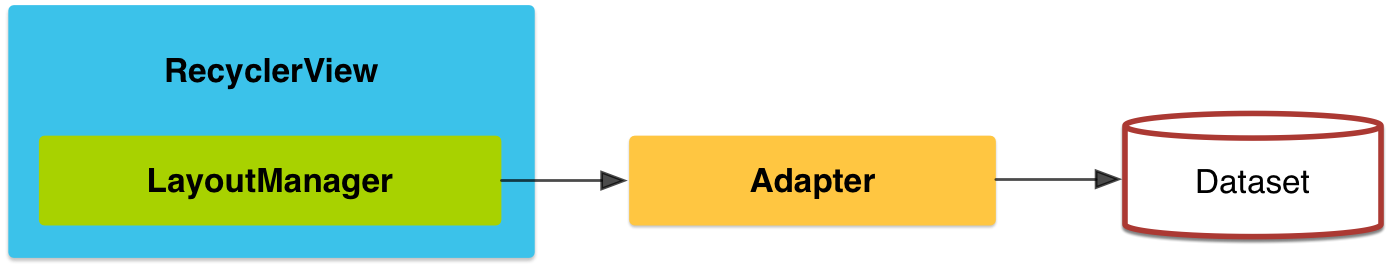
\includegraphics[width=\textwidth]{images/recycler/components.png}
	\caption{ RecyclerView is a major enhancement over ListView. It contains many new features like ViewHolder, ItemDecorator, LayoutManager, and SmoothScroller. But one thing that certainly gives it an edge over the ListView is; the ability to have animations while adding or removing an item. }
	\label{fig:recyclercomponents}
\end{figure}


\subsection{RecyclerView.Adapter}
RecyclerView uses an adapter to help convert our model data
into visual representations. A RecyclerView.Adapter  uses a generic to identify a ViewHolder that will be responsible for doing the work to actually tie
model data to row widgets.

RecyclerView.Adapter has three abstract methods that need to be implemented.

\begin{enumerate}
	\item getItemCount() , which fills the same role as does getCount() indicating how many items there will be in the RecyclerView
	\item onCreateViewHolder()  needs to create, configure,
	a ViewHolder for a particular row of our list. It is passed two parameters:
	\begin{enumerate}
		\item a ViewGroup that will hold the views managed by the holder, mostly for use
		with layout inflation, and
		\item an int that is the particular view type we are using, for cases where we have
		multiple view types
	\end{enumerate}
	\item onBindViewHolder()
	is responsible for updating a ViewHolder based upon the
	model data for a certain position .
\end{enumerate}

\subsection{ViewHolder}
The RecyclerView.ViewHolder is responsible for binding data as needed from our
model into the widgets for a row in our list. However, other than needing to use the base class of RecyclerView.ViewHolder ,
there is no other particular protocol that is mandated between the adapter and the
view holder. You can invent your own API.

This solution avoids all the findViewById() method calls in the adapter to find the views to be filled with data.

\subsection{LayoutManagers}
After adding a recyclerview to the activity, the first thing we do is call setLayoutManager() ,
which will associate a RecyclerView.LayoutManager with our RecyclerView, for example a LinearLayoutManager. RecyclerView
knows absolutely nothing about how to lay out its children. That work is delegated
to a RecyclerView.LayoutManager , so that different approaches can be plugged in as
needed.

There are three concrete subclasses of the abstract RecyclerView.LayoutManager
base class that ship with recyclerview-v7 :
\begin{enumerate}
	\item LinearLayoutManager , which implements a vertically-scrolling list
	\item GridLayoutManager ,
	which implements a two-dimensional vertically-
	scrolling list
	\item StaggeredGridLayoutManager , which implements a “staggered grid”, which
	has columns of cells like a GridView , but where the cells do not have to all
	have the same size.
\end{enumerate}


\subsection{ItemAnimator}
RecyclerView.ItemAnimator is a class that defines the animations performed on items and will animate ViewGroup changes such as add/delete/select notified to the adapter. DefaultItemAnimator is a basic animation available by default with the RecyclerView.

To customize the DefaultItemAnimator add an item animator to the RecyclerView. 


\subsection{Responding to Clicks}
Even though displaying elements in RecyclerView is better, in terms of performance, than its predecessors, ListView and GridView, it is not simple to add a clicklistener. 

To overcome this problem create an Interface

\begin{android}
public interface RecyclerViewItemClickListener {
	public void onClick(View view, int position);
	
	public void onLongClick(View view, int position);
}
\end{android}
To detect the item of the RecyclerView which is clicked we need a helper class.

\begin{android}
public class CustomRVItemTouchListener implements RecyclerView.OnItemTouchListener {
	
	//GestureDetector to intercept touch events
	GestureDetector gestureDetector;
	private RecyclerViewItemClickListener clickListener;
	
	public CustomRVItemTouchListener(Context context, final RecyclerView recyclerView, final RecyclerViewItemClickListener clickListener) {
		this.clickListener = clickListener;
		gestureDetector = new GestureDetector(context, new GestureDetector.SimpleOnGestureListener() {
			
			@Override
			public boolean onSingleTapUp(MotionEvent e) {
				return true;
			}
			
			@Override
			public void onLongPress(MotionEvent e) {
				//find the long pressed view
				View child = recyclerView.findChildViewUnder(e.getX(), e.getY());
				if (child != null && clickListener != null) {
					clickListener.onLongClick(child, recyclerView.getChildLayoutPosition(child));
				}
			}
		});
	}
	
	@Override
	public boolean onInterceptTouchEvent(RecyclerView recyclerView, MotionEvent e) {
		
		View child = recyclerView.findChildViewUnder(e.getX(), e.getY());
		if (child != null && clickListener != null && gestureDetector.onTouchEvent(e)) {
			clickListener.onClick(child, recyclerView.getChildLayoutPosition(child));
		}
		return false;
	}
	
	@Override
	public void onTouchEvent(RecyclerView rv, MotionEvent e) {
		
	}
	
	@Override
	public void onRequestDisallowInterceptTouchEvent(boolean disallowIntercept) {
		
	}
}
\end{android}

Basically what this class does is, detect the RecyclerView element under the (X, Y) position where the screen was clicked. This class is helpful for both click types created by the interface.


\section{CardView}
Cards are a popular visual metaphor in mobile development. Dividing content collections (or aspects of a larger piece of content) into cards makes it clearer how you can reorganize that content to fit various screen sizes and orientations. In some cases, you might have a single column of cards, while in other cases, you have cards
arranged more laterally.

In 2014, Google released cardview-v7 , another library in the Android Support
package, that offers a CardView . CardView is a simple subclass of FrameLayout ,
designed to provide a card UI, consisting of a rounded rectangle and a drop shadow.
In particular, CardView will use Android 5.0’s default drop shadows based on widget
elevation, while offering emulated drop shadows on earlier Android releases. This
way, you can get a reasonably consistent look going back to API Level 7.
To use this, you will have to add the cardview-v7 library to your app project.
Android Studio users can just add a dependency on the cardview-v7 artifact in the
Android Support repository

\section{Example}

\begin{example}
	In the repository found here \cite{Buysse2017}, we find an example demonstrating the principles explained above. Moreover, it makes use of a Fragment with a Recyclerview. It uses Butterknife as already demonstrated in previous example. For loading the images it makes use of the Picasso library (see \cite{Square2017}). 
\end{example}

\newpage
\section{Exercise}
\begin{exercise}
	Interview some of your classmates: ask their traits which describe them best. After the interview, make a nice picture (after asking permission of course).
	
	With this information in place, you should implement the following game: Guess who! If you don't know the game, see \cite{WikiHow2017}.
	
	The game should be able to be played in portrait and in landscape mode.
	Portrait mode should only contain a recyclerview with a small description of the student. The student should be able to be swiped out (i.e. he does not meet de traits). Pressing a student should show a new fragment with the student's description.
	Landscape mode should contain the list plus the description of the student. Swiping again deletes the student and the corresponding detailfragment.
	You should be able to restart the game.
	Make sure you apply the give best practices and try to animate as much as possible!
\end{exercise}

